\documentclass[a4paper,12pt]{article} 

%%% Работа с русским языком
\usepackage{cmap}                           % поиск в PDF
\usepackage{mathtext} 			 	       % русские буквы в формулах
\usepackage[T2A]{fontenc}               % кодировка
\usepackage[utf8]{inputenc}              % кодировка исходного текста
\usepackage[english,russian]{babel}  % локализация и переносы

%Матеша
\usepackage{amsmath,amsfonts,amssymb,amsthm,mathtools} % AMS
\usepackage{icomma} % "Умная" запятая

%\mathtoolsset{showonlyrefs=true} % Показывать номера только у тех формул, на которые есть \eqref{} в тексте.

%% Шрифты
\usepackage{euscript}	 % Шрифт Евклид
\usepackage{mathrsfs} % Красивый матшрифт

%% Свои команды
\DeclareMathOperator{\sgn}{\mathop{sgn}}

%% Перенос знаков в формулах (по Львовскому)
\newcommand*{\hm}[1]{#1\nobreak\discretionary{}
{\hbox{$\mathsurround=0pt #1$}}{}}

%%% Заголовок
\author{Злобина Вера Б02-002}
\title{Лабораторная работа 2.1.2

Определение $C_p / C_v$ методом адиабатического расширения}
\date{\today}

\begin{document}
	
\maketitle 
	
	
\newpage


\subparagraph*{Цель работы:}определение отношения $C_p / C_v$ углекислого газа  по измерения давления в стеклянном сосуде. Измерения производятся сначала после адиабатического расширения газа а затем после нагревания сосуда и газа до комнатной температуры. 
\subparagraph*{В работе используются:}стеклянный сосуд: U-образный жидкостный манометр; резиновая груша; газгольдер с углекислым газом. 

\begin{figure}[b!]	\label{plan2}
	
	\center{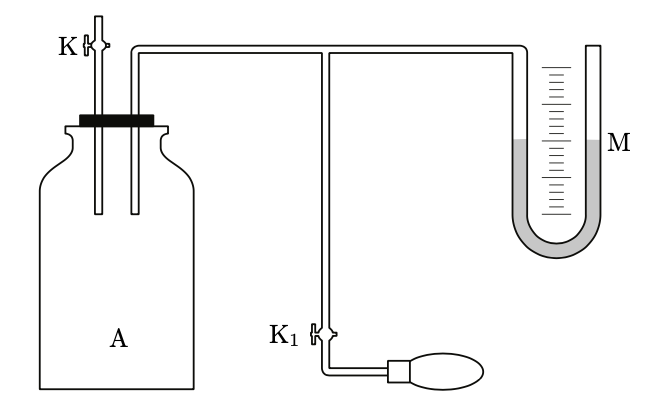
\includegraphics[width=1 \linewidth]{1.jpg}}
	\caption{Установка для определения $C_p / C_v$ методом адиабатического расширения газа}
	
\end{figure}



\subparagraph*{Экспериментальная установка.} Используемая для опытов экспериментальня установка состоит из стеклянного сосуда А (объёмом около 20 л), снабженного краном К, и U-образного жидкостного манометра, измеряющего избыточное давление газа в сосуде. Схема установки показана на Рис. 1. 

Избыточное давление создаётся с помощью резиновой груши, сосединённой с сосудом трубкой с краном $К_1$.

В начале опыта  в стеклянном сосуде А находится исследуемый газ при комнатной температуре $T_1$ и давлении $P_1$, несколько превышающем атмосферное давление  $P_0$. После открытия крана К, соединяющего сосуд А с атмосферой, давление и температура газа будут понижаться. Это уменьшение температуры приближённо можно считать адиабатическим. 

Для адиабатического процесса можно записать следующее уравнение: 

\begin{equation}\label{mk}
\left(\dfrac{P_1}{P_2}\right)^{\gamma - 1} = \left(\dfrac{T_1}{T_2}\right)^\gamma , 
\end{equation} 

где индексом "1" обозначено состояние после повышения давления в сосуде и выравнивания температуры с комнатной, а интексом "2"  $-$ сразу после открытия крана и выравнивания давления с атмосферным. 

После того, как кран К вновь отсоединит сосуд от атмосферы , происходит медленное изохорическое нагревание газа со скоростью, определяемой теплопроводностью стеклянных стенок сосуда. Вместе с ростом температуры растёт и давление газа. З время порядка $\Delta t_T$  (время установления температуры) система достигает равновесия, и установившаяся температура газа $T_3$ становится равной комнатной температуре $T_1$. 

Тогда используя закон Гей-Люссака для изохорического процесса и уравнение \eqref{mk} найдём $\gamma$:

\begin{equation}\label{acc}
\gamma = \dfrac{\ln(P_1 / P_0)}{\ln (P_1 / P_3)}.
\end{equation}

С учётом того, что $P_i = P_0 + \rho g h_i$ и пренебрегая членами второго порядка малости получим из \eqref{acc}:

\begin{equation}\label{r}
\gamma \approx \dfrac{h_1}{h_1 - h_2}.
\end{equation}


\newpage

\section*{Ход работы}

\subparagraph*{1.} Перед началом работы убедимся в том, что краны и места сочленений трубок достаточно герметичны. Для этого нужно наполнить баллон углекислым газом до давления, превышающего атмосферное  и перекроем кран $К_1$. По  U-образному манометру снимем зависимость давления $h$ в баллоне от времени $t$ и построим график зависимости $h = f(t)$. Из графика определим время установления термодинамического равновесия $\Delta t_T$. Стабильное избыточное давление воздуха $h_1$ в баллоне должно быть тщательно измерено. Как видно из полученного графика время установления равновесия составляет около 60 с. 


\begin{figure}[b!]	\label{plan2}
	
	\center{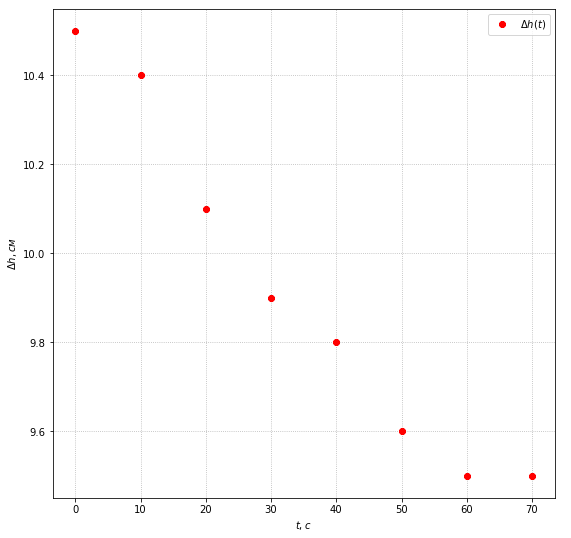
\includegraphics[width=1 \linewidth]{2.jpg}}
	\caption{График зависимости $h(t)$}
	
\end{figure}



\subparagraph*{2.} Откроем кран К на короткое время и закроем его снова. Подождём, пока уровень жидкости в манометре перестанет изменяться. Это произойдёт, когда температура газа в сосуде сравняется с комнатной, примерно через время $\Delta t_T$. Запишем разность уровней жидкости в манометре $h_2$. Проведём серию из 5--8 измерений сначала для времени открытия крана $\Delta t = 0,5 с$, а затем для $\Delta t \approx 1,0 с и \Delta t \approx 1,5 с$. По полученным данным вычислим используя формулу \eqref{r} вычислим $\gamma$ и построим график зависимости $\gamma(\Delta t)$ (График 1).






\begin{table}[h!] 
	\caption{Экспериментальные данные для $\Delta t = 0,5$}
	\begin{center}
	\begin{tabular}{|*{4}{l|}}
		\hline
	№ & $h_1$ , см & $h_2$, см & $\gamma$ \\ \hline
	1& 9.6& 1.5 & 1.185 \\ \hline
	2 & 9.1 & 1.4 & 1.181 \\ \hline
	3 & 9.2 & 1.5 & 1.194 \\ \hline
	4 & 9.3 & 1.5 & 1.182 \\ \hline
	5 & 9.1 & 1.4 & 1.181 \\ \hline 
	6 & 9.2 & 	1.5 & 1.195 \\ \hline
	7 & 9.2 & 1.4 & 1.179 \\ \hline 
	& & $\gamma_{ср} = 1.187 $ & $\sigma_{с, \gamma} = 0.002$ \\ \hline
	\end{tabular}
	\end{center}
\end{table}

Как видно из предварительных вычислений случайная погрешность $\gamma$ очень мала в сравнении с инструментальной (которая оценочно будет на порядок больше). 



\begin{table}[h!] 
	\caption{Экспериментальные данные для $\Delta t = 1,0$}
	\begin{center}
		\begin{tabular}{|*{4}{l|}}
			\hline
			№ & $h_1$ , см& $h_2$, см & $\gamma$ \\ \hline
			1 & 9.1 & 1.2 & 1.152 \\ \hline
			2 & 8.7 & 1.2 & 1.160 \\ \hline 
			3 & 9.0 & 1.2 & 1.154 \\ \hline
			4 & 9.0 & 1.2 & 1.154 \\ \hline
			5 & 9.0 & 1.2 & 1.154 \\ \hline
			& & $\gamma_{ср} = 1.155 $ & $\sigma_{с, \gamma} = 0.003$ \\ \hline
		\end{tabular}
	\end{center}
\end{table}



\begin{table}[h!] 
	\caption{Экспериментальные данные для $\Delta t = 2,0$}
	\begin{center}
		\begin{tabular}{|*{4}{l|}}
			\hline
			№ & $h_1$, см & $h_2$, см & $\gamma$ \\ \hline
			1 & 9.1 & 1.0 & 1.123 \\ \hline 
			2 & 8.8 & 0.9 & 1.114 \\ \hline
			3 & 8.9 & 1.0 & 1.127 \\ \hline 
			4 & 8.8 & 1.0 & 1.128 \\ \hline
			5 & 8.8 & 1.0 & 1.128 \\ \hline
			6 & 9.1 & 1.0 & 1.123 \\ \hline 
			& & $\gamma_{ср} = 1.124 $ & $\sigma_{с, \gamma} = 0.007$ \\ \hline			
		\end{tabular}
	\end{center}
\end{table}


Теперь оценим вклад приборной погрешности при вычислении величины $\gamma$. Измерения $h_1$  и $h_2$ проводились с точностью 1мм. Пользуясь формулой \eqref{r} можно получить, что относительная погрешность искомой величины $$\dfrac{\sigma_\gamma}{\gamma} = \sqrt{\left(\dfrac{\partial\gamma(h_1, h_1 - h_2)}{\partial h_1}\sigma_{h_1}\right)^2 + {\left(\dfrac{\partial\gamma(h_1, h_1 - h_2)}{\partial h_1 - h_2}\sigma_{h_1 - h_2}\right)^2} }\approx 0.03$$

что даёт нам право пренебречь статистической погрешностью $\gamma$.


Точность измерения времени, в течение которого газ выпускался из сосуда, оценивается точностью моей реакции, опыт показал, что эта величина составляет около 0.1 или даже меньше (поскольку интервал в 0.5 с примерно с такой точностью совпадает с временем прокручивания крана на полоборота), поэтому можно считать, что время измерено с точностью $\approx 7\%$

Тогда итоговая погрешность измерения показателя адиабаты составляет около $\sqrt{0.03^2+0.07^2} = 8\%$

	\begin{figure}[h!]	\label{plan2}
	
	\center{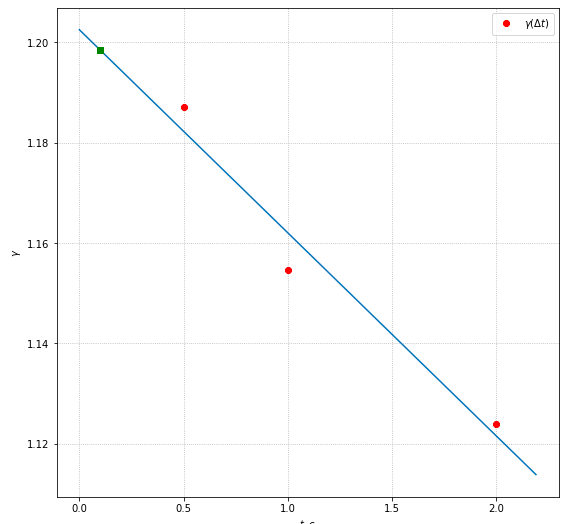
\includegraphics[width=1 \linewidth]{3.jpg}}
	\caption{График зависимости $\gamma(\Delta t)$}
	
\end{figure}

\subparagraph*{3.} Окончательный результат следует получить экстраполяцией зависимости $\gamma$ от $t$ примерно к значению $\Delta t = 0,1 - 0,2 с$, когда давление уже почти сравнялось с атмосферным, но теплопроводность ещё не так сильно повлияла на уменьшение $\gamma$. Из полученного графика (на графике данная точка отмечена зелёным квадратом) можно сделать вывод, что $\gamma_{CO_2} = 1.20 \pm 0.10$. В то время как табличное значение $\gamma_{CO_2} = 1.30$, т. е. совпадает с полученным значением в пределах погрешности. 


	
	
\newpage
	
\section*{Вывод}


В ходе эксперимента было получено значение показателя адиабаты, которое в пределах погрешности совпадает с табличным. Что говорит о том, что экстраполяция данных на значения, когда теплообмен ещё не успел внести большой вклад, позволяет получить правильный решультат. На больших временах был замечен этот вклад, что отображалось сильным занижением величины $\gamma$ вплоть до порядка 1.1.

\end{document}
